\section{Container Linux Alpine}

No primeiro exercicio pretende-se criar um container que tenha a port 9999 do container mapeada para a port 8668 do host. Também pretende-se criar um bind mount que mapeia uma diretoria do container numa diretoria do host.

Para tal executou-se o comando seguinte:

\begin{lstlisting}

docker run -it --name alpine-container \
-v /home/apocas/docker_dir:/home/internal_dir \
-p 8668:9999 alpine:latest /bin/ash

\end{lstlisting}

O comando dá o nome de alpine-container ao container que foi criado, mapeando a diretoria (\"\-v\") \emph{home/apocas/docker\_dir} do host para a diretoria \emph{/home/internal\_dir} dentro do conatiner. Os ports foram mapeados com a opção (\"\-p\"). Finalmente, vai-se buscar a última versão da imagem do Alpine correndo o programa ash que corresponde ao intrepretador de comandos default do Sistema Operativo.

\section{Volumes}

Nesta questão pretende-se criar um volume com o nome \"my\-volume\-1\" para tal executou-se o comando:

\begin{lstlisting}

docker volume create my-volume-1

\end{lstlisting}

Também se pretende saber qual é o mountpoint (local onde o volume faz as persistências) e o driver(Qual o host onde se vai montar) do mesmo. Para tal, executou-se o comando:

\begin{lstlisting}

docker volume inspect test-vol

\end{lstlisting}

O resultado obtido do mesmo foi

\begin{lstlisting}

[
    	{
        	"CreatedAt": "2020-02-20T11:02:31Z",
        	"Driver": "local",
        	"Labels": {},
        	"Mountpoint": "/var/lib/docker/volumes
        	/my-volume-1/_data",
        	"Name": "my-volume-1",
        	"Options": {},
        	"Scope": "local"
    	}
	]


\end{lstlisting}

A partir do resultado podemos retirar que o mountpoint é \emph{ /var/lib/docker/volumes/my-volume-1/\_data }
e que o Driver é \emph{\"local\"}.

\section{Bridge Network}

A partir de dois containers criados manualmente, pretende-se inspecionar a Bridge Network para verificar os IPs dos mesmos e se é possível comunicar-se entre eles. 

Antes de proceder a inspeção da Bridge Network criada por defeito, criou-se dois containers através dos comandos:

\begin{lstlisting}

docker run -dit --name container1 ubuntu:latest /bin/bash

docker run -dit --name container2 ubuntu:latest /bin/bash
	
\end{lstlisting}

Sabendo que os IDs devolvidos para cada um deles são, 
\begin{lstlisting}

"01fb17f6ffd6a4ba02395719351d8a89b4d3d81047d854beddc987dcf904bbfb"

"2f2005b7c527e5c4656a6c023b8b5b4731eedf97fd8d9da5bfa181f1c757aa72"

\end{lstlisting}
Para inspecionar recorreu-se ao comando:

\begin{lstlisting}

docker network inspect bridge

\end{lstlisting} 

Obtendo-se o resultado que está na próxima figura:

\begin{figure}[H]

	\centering

 	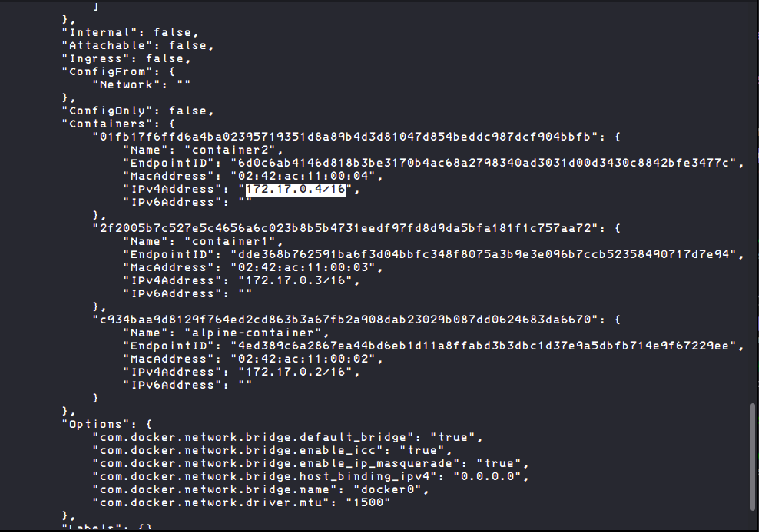
\includegraphics[width=\textwidth]{BridgeIPs.png}

 	\caption {Bridge Network}

  	\label {fig:Brid}
\end{figure}

Pode-se constatar os IPs dos container associados as redes locais \emph{172.17.0.4/16} e \emph{172.17.0.3/16}.

Respondendo a questão da comunicação entre eles pode-se se constatar que , como dito no próprio, não se pode comunicar entre eles por nome visto que não estão na mesma network. No entanto, é possível comunicar usando os IPs do comando anterior como está representado na figura seguinte.

\begin{figure}[H]

	\centering

 	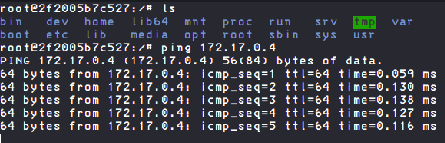
\includegraphics[width=\textwidth]{PingBridge.png}

 	\caption {Comunição por IP através da Bridge Network}

  	\label {fig:Brid}
\end{figure}

\section{Manual Network}

Neste exercicio pretende-se criar uma Network para juntar os dois containers e, verificar se já é possível pingar-se entre eles usando os nomes.

Para criar a rede com nome \"my-network-1\" utilizou-se o comando:

\begin{lstlisting}

docker network create my-network-1

\end{lstlisting}

No caso de se quiser começar un novo container pode-se fazer:

\begin{lstlisting}
	
docker run -dit --name container3 --network my-network-1 ubuntu:latest 
/bin/bash

\end{lstlisting}
	
	Assim cria-se un container a correr o Ubuntu em modo Daemon usando a bash como comando default ligando-o a network criada anteriormente.
	
	Caso estivesse já correr os containers pode-se fazer:

\begin{lstlisting}
	
docker network connect my-network-1 container1

\end{lstlisting}

Para inspecionar e encontrar mais informações sobre a network criada utiliza-se o comando:

\begin{lstlisting}

docker network inspect my-network-1

\end{lstlisting}

Pode descobrir-se que qual o IP da subrede criada, como tambem os IPs dos container ligados a mesma.
	Tambem é possivel descobrir qual o Driver que esta network está a usar, quando foi criada e o seu nome.

\begin{figure}[H]

	\centering
	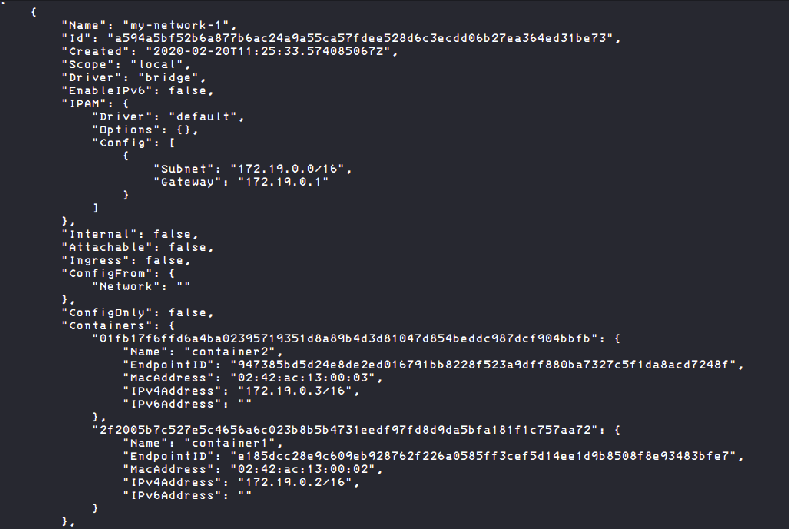
\includegraphics[width=\textwidth]{NetworkManual.png}

 	\caption {Resultado do Inspect da Network}

  	\label {fig:sNet}
\end{figure}

A comunicação dos containers ligados a network criada manualmente, pode ser feita através dos nomes dos mesmos como se pode ver na figura seguinte. Aqui o Container com ID \"1f...\" comunica com o Container de nome \"container1\".

\begin{figure}[H]

	\centering
	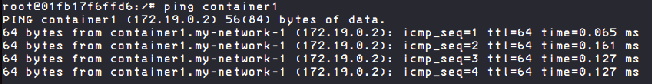
\includegraphics[width=\textwidth]{PingNet.png}

 	\caption {Ping aos Containers por Nome}

  	\label {fig:NomeNet}
\end{figure}

\section{Analise de Comandos após Docker-Compose}

Nesta seção pretende-se após executar o docker-compose(docker-compose -d) que se encontra na seção 2 do enunciado analisar o que este fez. Após a execução pode ver-se que foi criada a network \"ex5\_container-net\" e o volume \"ex5\_httpd-vol\". Os valores do volume e da network criada foram os default que normalmente são postos quando criados normalmente. 

\begin{figure}[H]

	\centering
	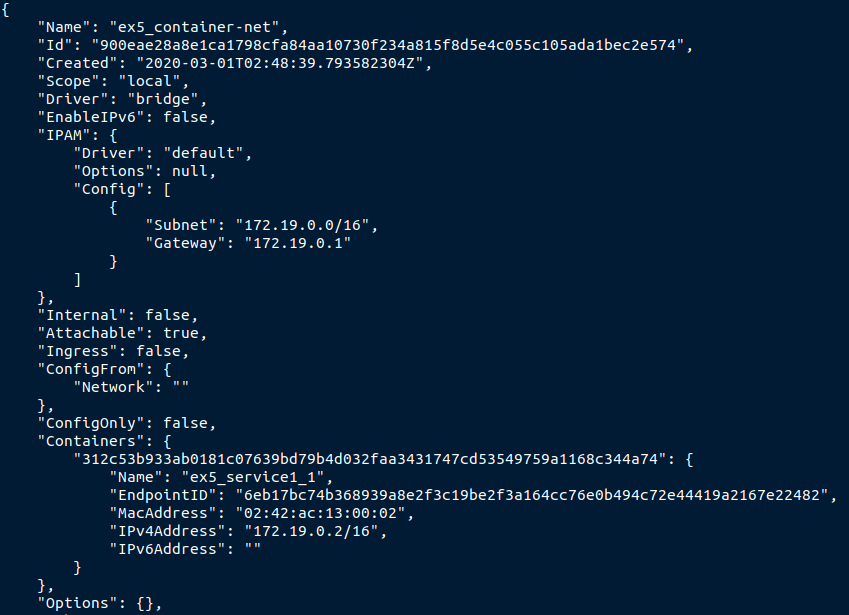
\includegraphics[width=\textwidth]{networkInspect.png}

 	\caption {Resultado do Inspect da Network após o Docker-Compose}

  	\label {fig:ComposeNetInsp}
\end{figure}

\begin{figure}[H]

	\centering
	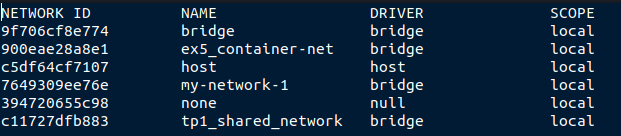
\includegraphics[width=\textwidth]{networkLS.png}

 	\caption {Resultado do LS das Networks após o Docker-Compose}

  	\label {fig:ComposeNetLs}
\end{figure}

\begin{figure}[H]

	\centering
	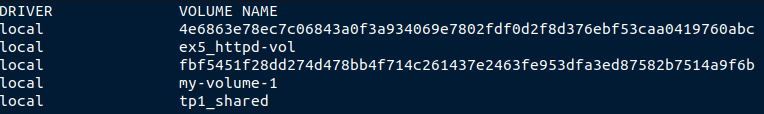
\includegraphics[width=\textwidth]{volumeLS.png}

 	\caption {Resultado do LS dos Volumes após o Docker-Compose}

  	\label {fig:ComposeVol}
\end{figure}

\begin{figure}[H]

	\centering
	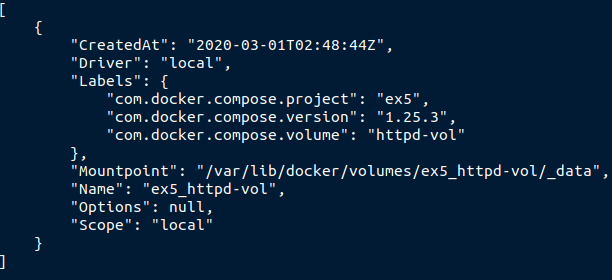
\includegraphics[width=\textwidth]{volumeInspect.png}

 	\caption {Resultado do Inspect do Volume após o DockerCompose}

  	\label {fig:ComposeVolInsp}
\end{figure}

\section{Docker-Compose criado}

No exercicio pretende-se criar um ficheiro Docker-Compose que comece pelo menos dois serviços que estão na mesma Network, partilham um volume, um dos serviços tambem têm um bind mount, um dos serviços tem que ter a porta 9999 exposta na 8888 do host.

O seguinte Docker-Compose foi criado:

\begin{figure}[H]

	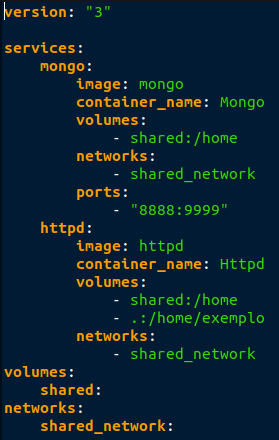
\includegraphics[scale=0.3]{DockerCompose.png}
	\centering

 	\caption {Docker-Compose}

  	\label {fig:DocCom}
\end{figure}

Este Docker-Compose inicia dois containers:

\begin{itemize}

\item Uma imagem Mongo num container com nome Mongo que tem persistência num volume shared que vai ser criado pelo Docker-Compose.Também coneta-se a uma network que vai ser criada nesse mesmo ficheiro.Finalmente, mapeia-se a porta do host 8888 para a porta do container 9999.

\item Uma imagem HTTPD com nome Httpd utilizando para persistência o mesmo volume que o Mongo e mais um bind mount da pasta atual para uma pasta /home/exemplo e está conetado a mesma Network do Mongo.

\end{itemize}

Observando os resultados dos comandos \"inspect\" e \"ls\" obtemos que os containers foram criados, o volume também,como também o bind e as portas abertas.

\section{DockerFile}

No Docker file foi definido primeiramente a imagem base, ubuntu. De seguida foi definido o maintainer. Com o RUN atualizamos os pacotes da imagem e instalamos o nginx que é um server HTTP e proxy reverso. Com o Expose expomos a porta do container e por fim com o CMD informamos qual o comando que será executado depois de ser feita a criaçao do container. Alem disto se usasse-mos o ENTRYPOINT podemos fazer uso do comando anterior para definir parâmetros que este usar.

\begin{figure}[H]

	\centering
	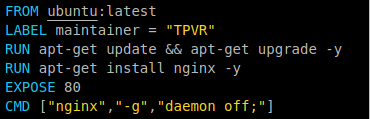
\includegraphics[width=\textwidth]{dockerFile.png}

 	\caption {DockerFile}

  	\label {fig:DocCom1}
\end{figure}

Apos criado o DockerFile foi necessario fazer build do mesmo. Usamos o comando:
docker build -t tpvr/nginx:1.0 .

\begin{figure}[H]

	\centering
	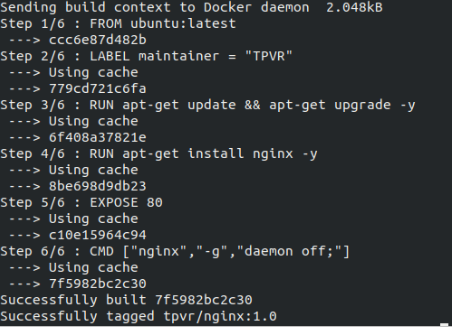
\includegraphics[width=\textwidth]{dockerFile2.png}

 	\caption {Steps do Docker File}

  	\label {fig:DocCom2}
\end{figure}


Como é possível observar na imagem acima, foi criada uma imagem “espelhada” do ubuntu e com o nginx instalado, entre outros pacotes. Com o comando docker imagens provamos uma vez mais que esta foi criada.

\begin{figure}[H]

	\centering
	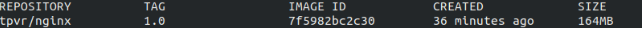
\includegraphics[width=\textwidth]{dockerFile3.png}

 	\caption {Image Criada}

  	\label {fig:DocCom3}
\end{figure}


De seguida, foi necessario testar e para isso criamos um container 

\begin{figure}[H]

	\centering
	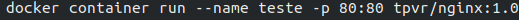
\includegraphics[width=\textwidth]{dockerFile4.png}

 	\caption {Comando para correr a Imagem}

  	\label {fig:DocCom4}
\end{figure}

E por fim podemos observar que ao abrir localhost:80 este direciona-nos para a pagina inicial do nginx, como mostra a figura abaixo.

\begin{figure}[H]

	\centering
	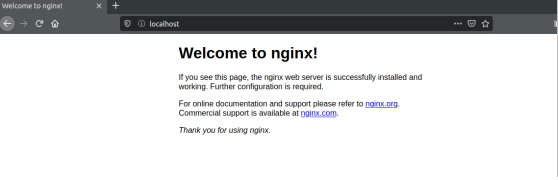
\includegraphics[width=\textwidth]{dockerFile5.png}

 	\caption {Serviço NGINX}

  	\label {fig:DocCom5}
\end{figure}



\section{Build Automática}

A build automática pode ser feita seguindo o link seguinte \href{https://hub.docker.com/r/kaiserfrost/tp1?fbclid=IwAR2Lz_-7bJ2MdjYj38VvFP2TxxP3n-LMpGkPUi5sURwsbloGhXOCwPnaxqQ}{Imagem}

\begin{lstlisting}

https://hub.docker.com/r/kaiserfrost/tp1
?fbclid=IwAR2Lz_-7bJ2MdjYj38VvFP2TxxP3n-LMpGkPUi5sURwsbloGhXOCwPnaxqQ

\end{lstlisting}
